\section{系统实现}

\subsection{前台展示功能实现}

\subsubsection{首页页面实现}

进入到智慧工厂管理系统的首页,首先向客户或者供应商展示公司介绍,第一个页面有公司标语和简短介绍等;在上方的导航栏有一些功能按钮,例如工厂特点介绍、提供的服务、工厂的特点、联系方式和管理员登录入口等。

导航栏部分使用div元素进行包装,使用定义好的css样式进行修饰。在导航栏下方展示工厂企业的口号标语以及简单的业务介绍,使用div元素将整体进行封装,根据不同的内容展示使用各自的css样式。系统的前台展示如图\ref{fig:index}所示。通过首页页面向客户展示工厂标语以及服务介绍;向客户进一步介绍工厂服务内容以及服务特点情况;向客户展示工厂生成环境图片,当鼠标移到图片上可进一步显示图片内容介绍;最后向客户提供工厂的联系方式等信息。

\begin{figure}[H]
    \centering
    \begin{subfigure}{.45\textwidth}
        \centering
        
\includegraphics[width=\textwidth]{figures/5index.png}
        % \subcaption{系统首页展示图}
        % \label{fig:index1}
    \end{subfigure}
    \qquad
    \begin{subfigure}{.45\textwidth}
        \centering
        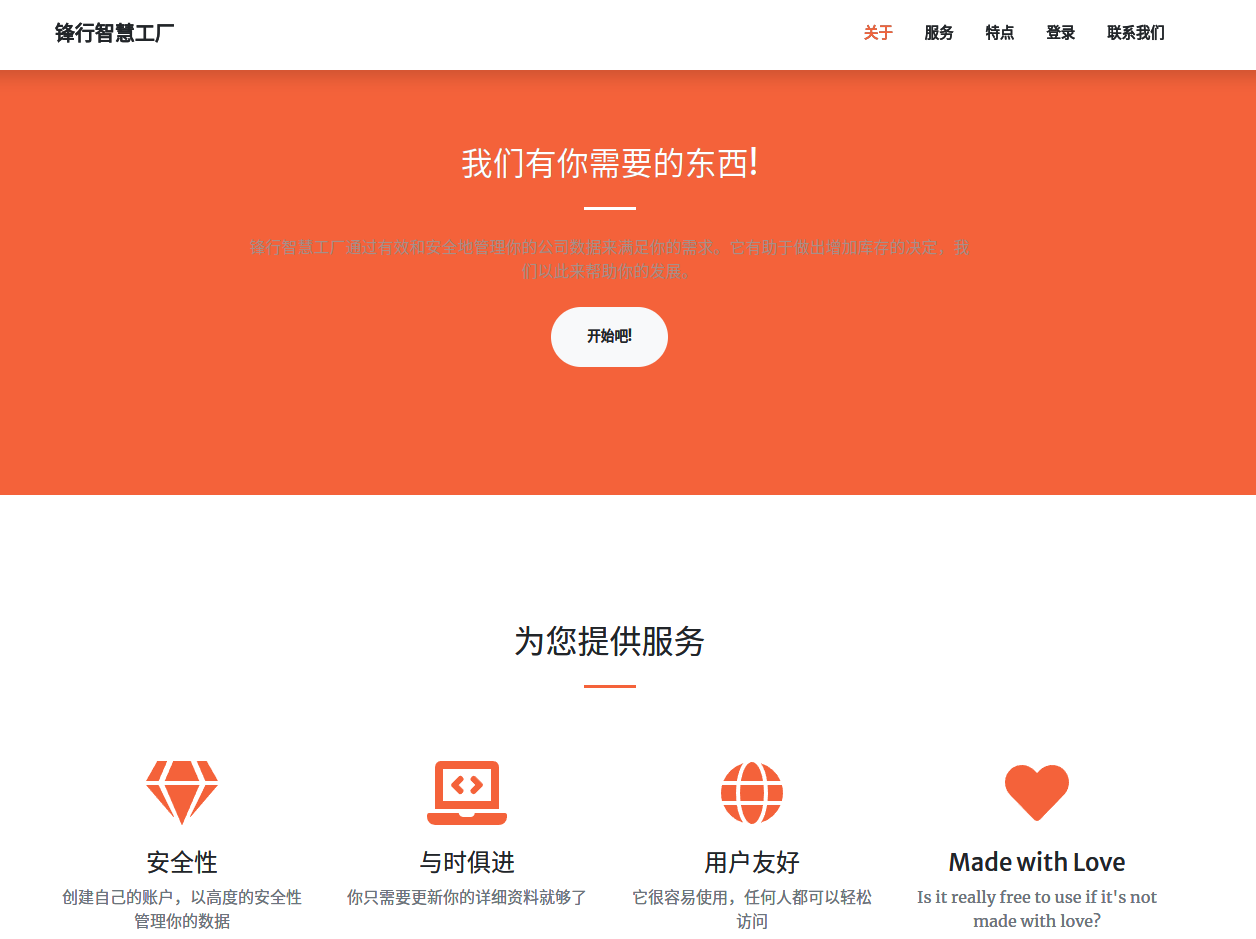
\includegraphics[width=\textwidth]{figures/5index2.png}
        % \subcaption{工厂服务特点图}
        % \label{fig:index2}
    \end{subfigure}
    \\
    \begin{subfigure}{.45\textwidth}
        \centering
        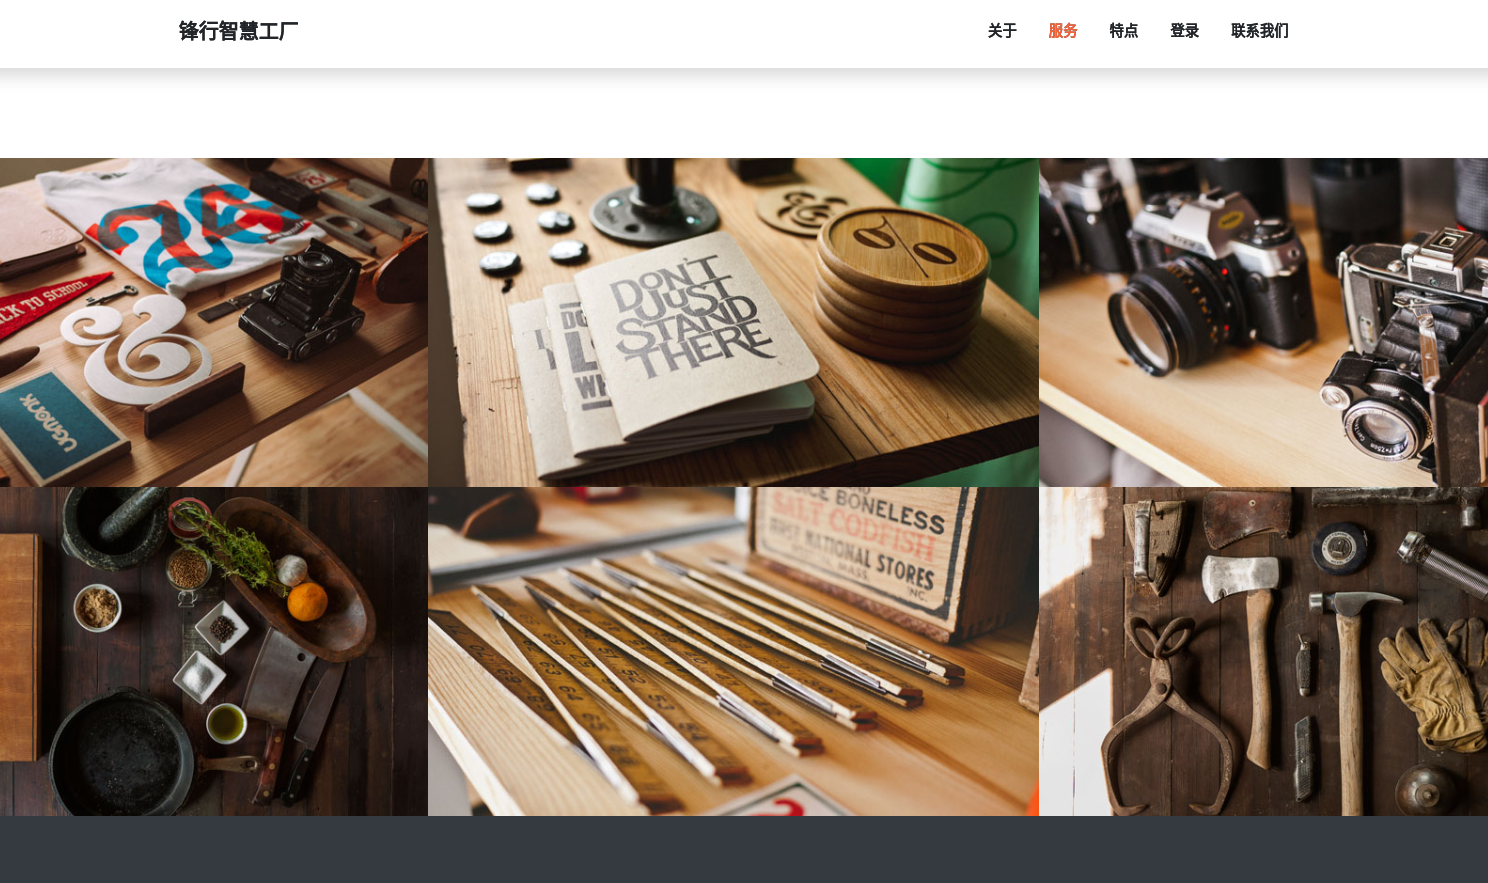
\includegraphics[width=\textwidth]{figures/5index3.png}
        % \subcaption{工厂介绍图片页面图}
        % \label{fig:index3}
    \end{subfigure}
    \qquad
    \begin{subfigure}{.45\textwidth}
        \centering
        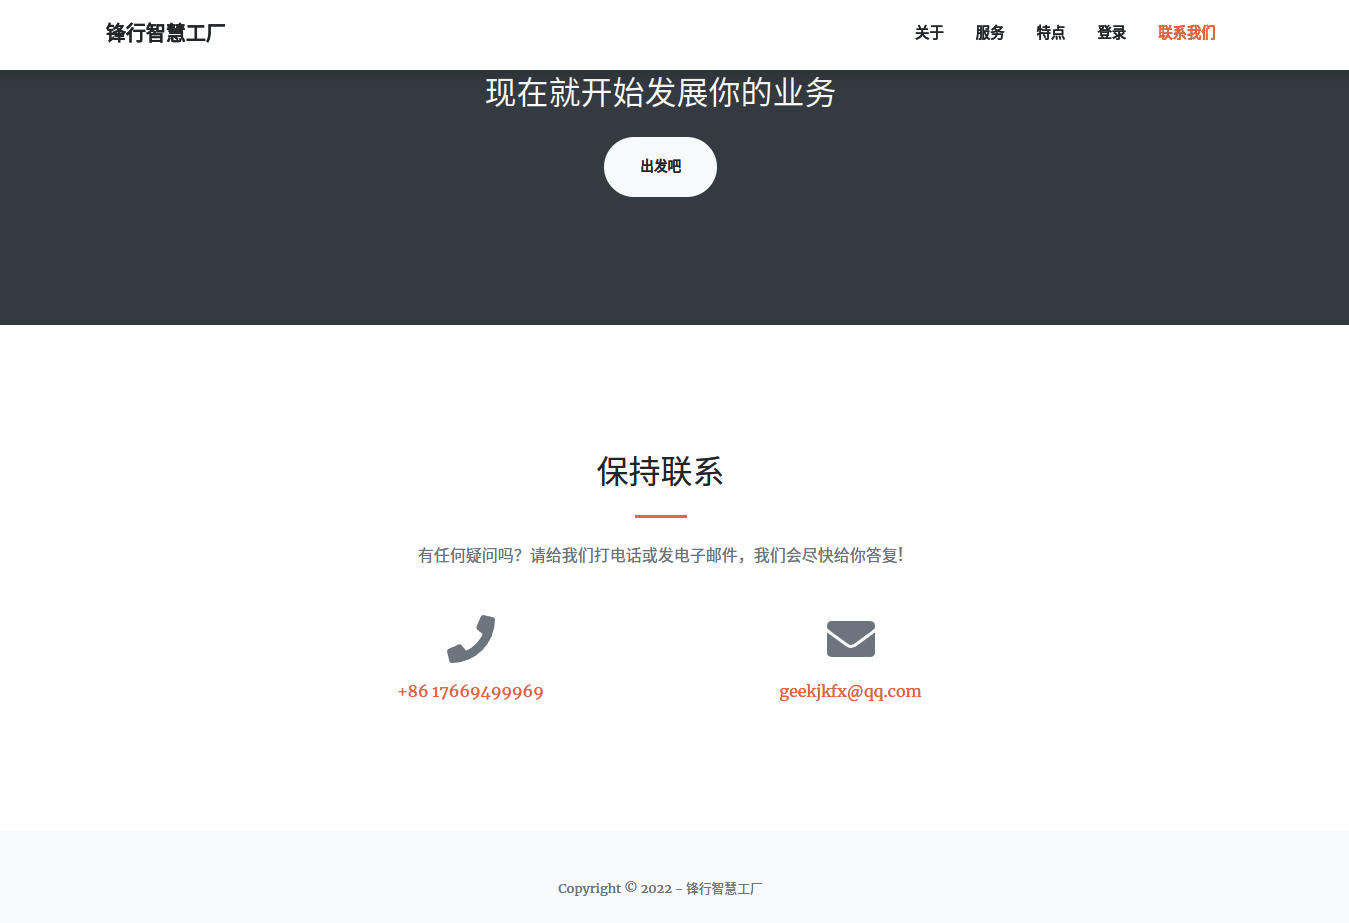
\includegraphics[width=\textwidth]{figures/5index4.png}
        % \subcaption{工厂联系方式页面图}
        % \label{fig:index4}
    \end{subfigure}
    \caption{前台页面展示图}
    \label{fig:index}
\end{figure}

\subsubsection{登录注册页面实现}

系统首页除展示完工厂介绍之外,在上方导航栏位置处还有登录按钮供工厂管理人员对工厂信息进行管理入口。

在登录注册页面,首先定义好css样式,对body元素、a标签以及一些自定义类css选择器进行样式美化,使用Django的模板(template)模块,继承base基页面,使用模板语言检测当前页面是否存在后端传来的消息提示,使用模板语言进行展示。本系统将登录和注册功能放置与同一页面,用户可通过点击不同功能的按钮进行选择登录或注册功能,并且使用input标签元素获取用户输入,将输入好的信息通过POST请求发送至后端处理。在后端view视图模块中,处理来自于前台账号信息表单的HTTP请求,分别获取到POST表单中的账号信息,使用正则表达式检查输入字符串中是否包含特殊字符并进行提示。之后,使用数据访问对象新建一个用户实例,并且将输入信息设置为属性,将账号实例进行持久化操作保存至数据库。在HTTP的响应中,根据账号信息输入是否合法以及账号注册成功与否的消息返回至前台并进行展示。如图\ref{fig:loginregisterf}所示,在后台登录页面,管理人员输入管理账号与密码进行登录。工厂的某一个部门组织可以在注册页面注册管理账号,并且填写组织名称、电子邮件、电话号码、登录用户名以及密码等信息。

\begin{figure}[H]
    \centering
    \begin{subfigure}{.45\textwidth}
        \centering
        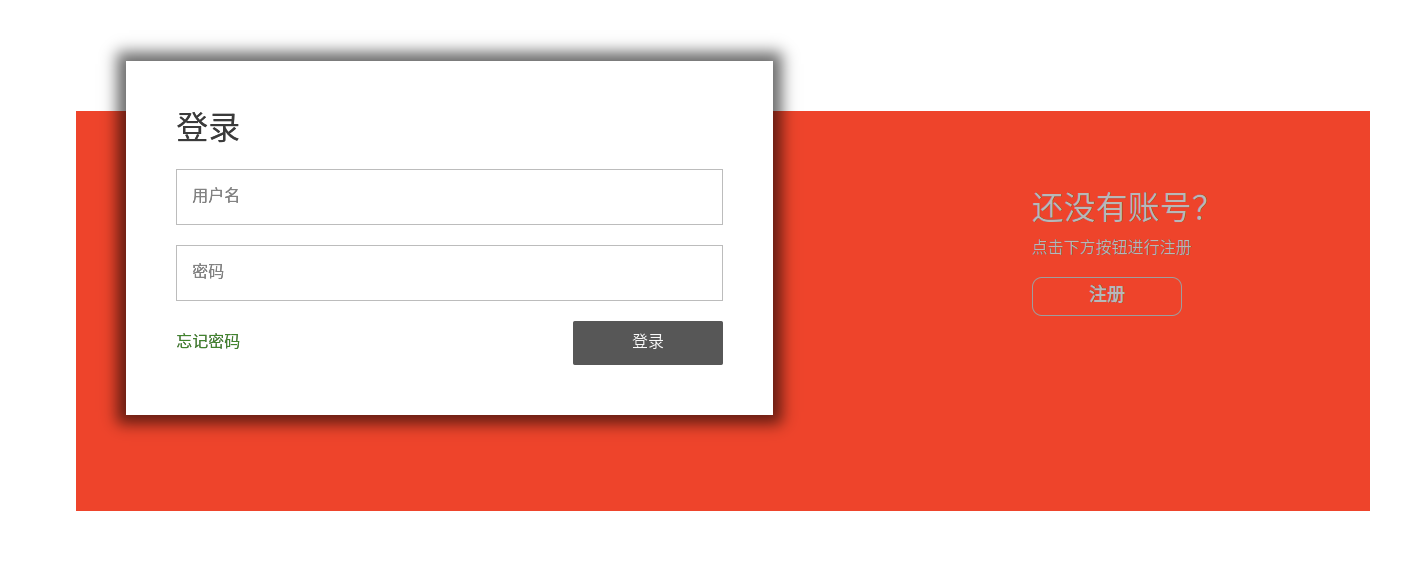
\includegraphics[width=\textwidth]{figures/5login.png}
        % \subcaption{登录页面图}
        % \label{fig:loginpage}
    \end{subfigure}
    \qquad
    \begin{subfigure}{.45\textwidth}
        \centering
        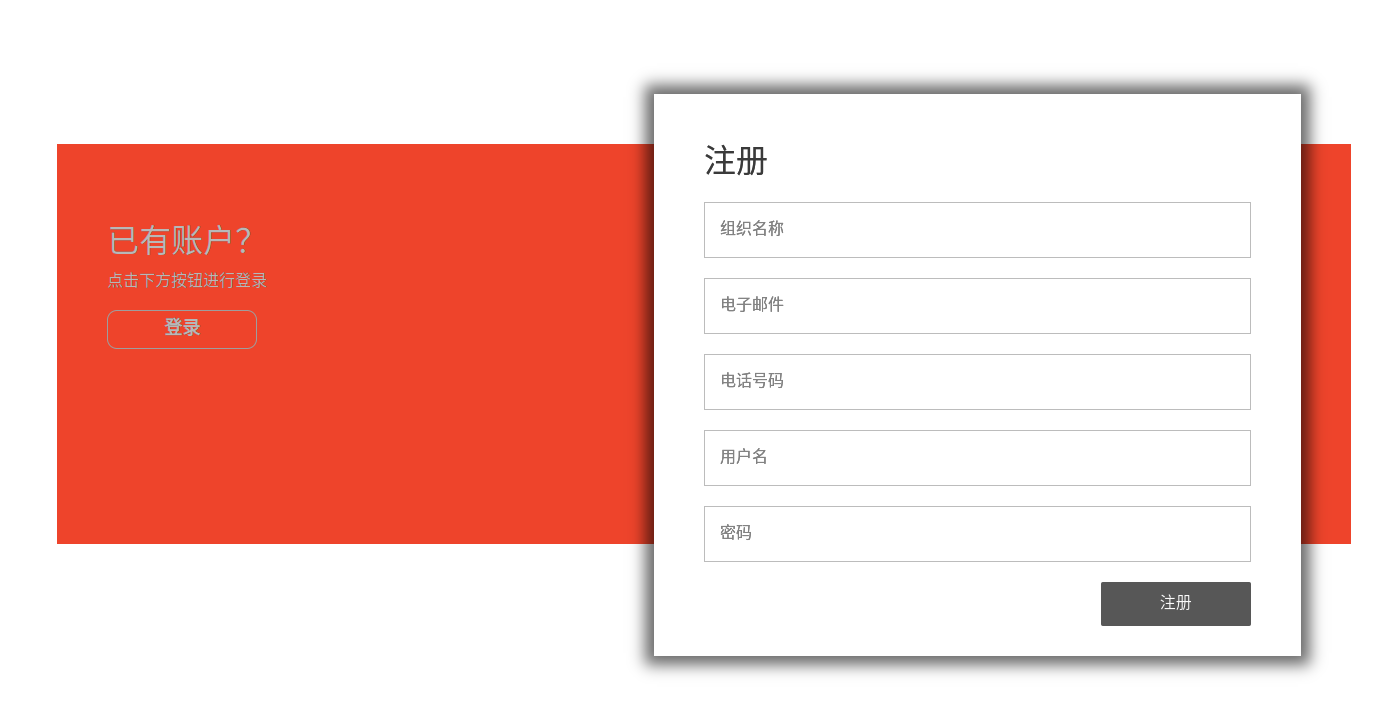
\includegraphics[width=\textwidth]{figures/5register.png}
        % \subcaption{注册页面图}
        % \label{fig:register}
    \end{subfigure}
    \caption{登录注册页面图}
    \label{fig:loginregisterf}
\end{figure}

\subsection{后台管理功能实现}

\subsubsection{后台仪表盘功能实现}

当工厂部门组织管理员登录到后台管理页面,首先向管理员展示仪表盘页面,该仪表盘可以从工厂各个角度展示工厂当前部门组织的交易情况。首先使用div标签仪表盘页面整体框架构建好,根据仪表盘所展示的页面内容,使用不同的div.class类别,将财务状况、月度收益、年度收益以及交易记录所要展示的内容分派到不同的div标签中。之后,使用Chart.js的JavaScript脚本创建出不同类别的可视化图形的对象。创建一个Chart类实例,输入绘图类型为doughnut饼图,使用Django的模板语言获取到后端数据,将当前部门的月度收益状况输入,并且根据输入和支出指派两个标签,并且绘制不同的颜色生成一个饼图,放置与月度收益概览的div元素中。在年度输入概览中,创建一个Chart类实例,输入类型为line折线图,以同样的方式获取后端数据生成折线图,放置于div元素中。

在账户收入支出部分,在前台页面使用模板语言获取后端传来的账户金额数据,在div标签元素中进行展示。在后端views请求处理方法中,首先在交易记录的实体表中,使用数据访问对象以月为组进行聚合过滤,获取到每个月的收入和支出数据,并且计算出每个月的利润数据,封装至字典对象中,通过HTTP响应发送到前端。并且根据当前发起请求的时间,查询数据得到当前月份的财务状况,展示到仪表盘页面上方。仪表盘页面的下方,向工厂部门管理人员展示最近的入账和出账交易记录,使用数据访问对象获取到当前月份的交易记录实例,通过HTTP响应返回至前端进行展示。

\begin{figure}[H]
    \centering
    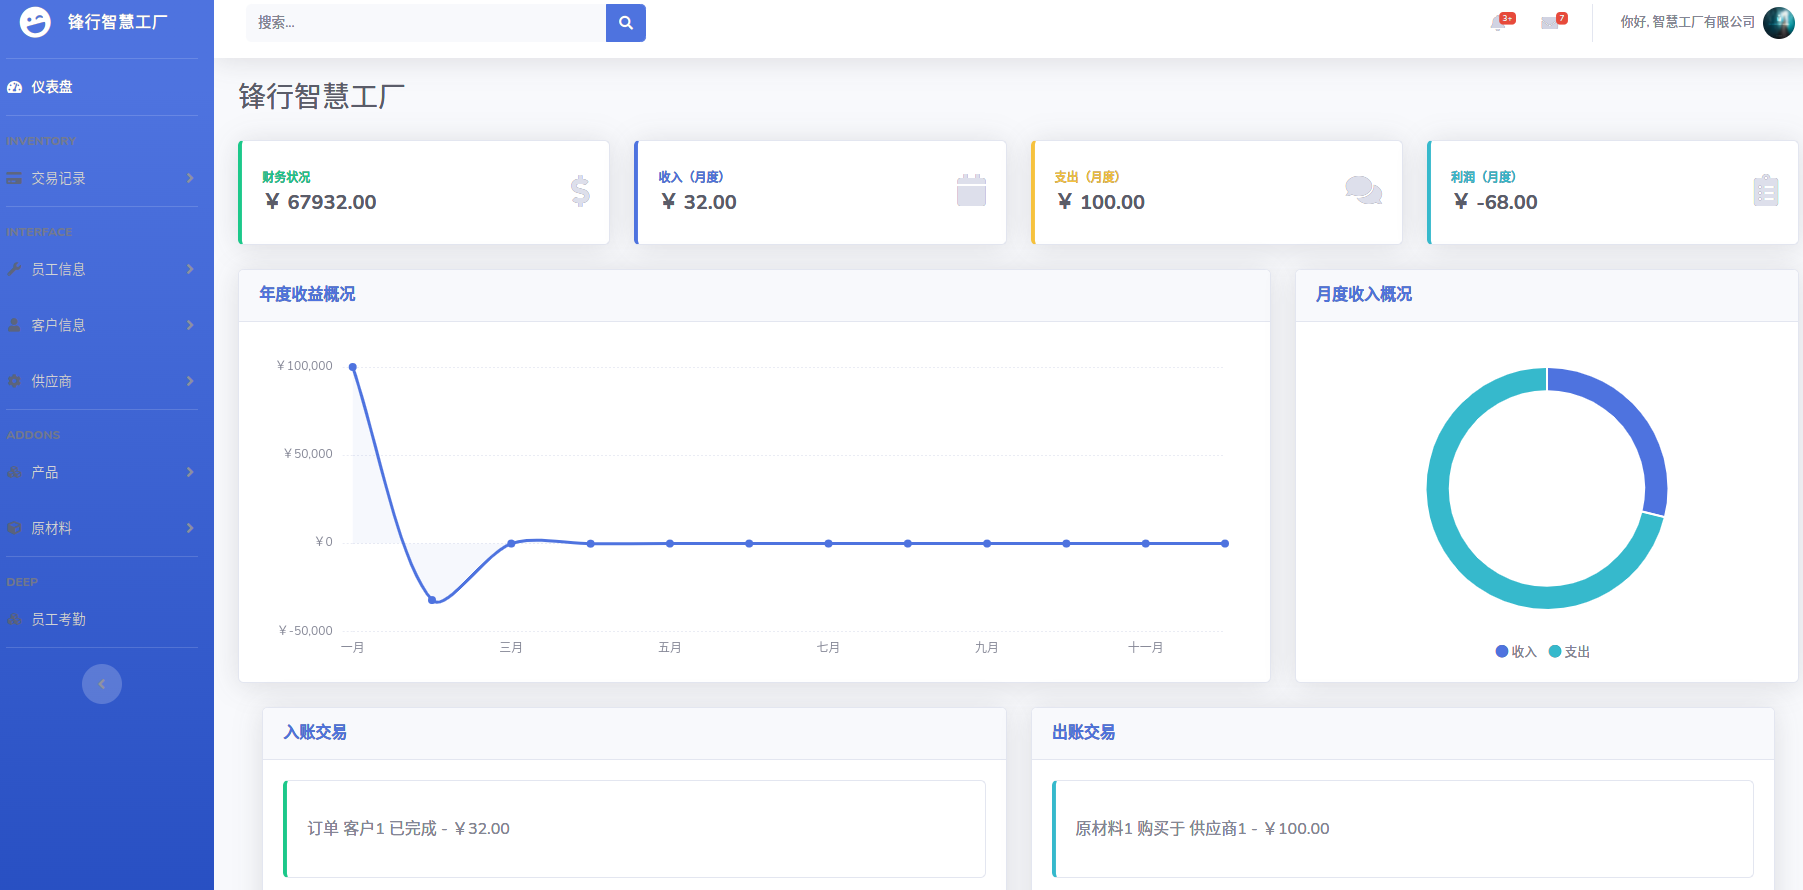
\includegraphics[width=.75\textwidth]{figures/5dashboard.png}
    \caption{后台仪表盘页面图}
    \label{fig:dashboard}
\end{figure}

如图\ref{fig:dashboard}所示,后台首页页面左方一栏是后台管理功能导航栏;右上方为当前登录部门组织账号概览;仪表盘页面第一行为当前组织部门财务状况的数字展示,其中包括财务状况和月度的收入、支出以及利润信息;第二行为当前组织部门的财务状况的可视化展示,包括年度收入支出的折线图以及月度收入支出的饼图;在最下方,向管理员展示最近的交易记录,左部分展示入账的交易记录,右方展示出账的交易记录。

\subsubsection{人员信息管理功能实现}

在工厂管理员进入到后台管理页面之后,在左方的导航栏处排列了各种工厂信息管理的页面按钮。其中包括交易记录、员工信息、客户信息、供应商信息、产品信息、原材料信息和员工考勤按钮,点击特定导航栏按钮,可以展开二级菜单展示当前信息管理的各种操作。点击特定导航栏按钮之后展开的人员管理类的信息管理操作,展示了员工信息的信息管理操作,其中包括查看员工、添加员工以及支付薪资按钮操作。

% \begin{figure}[H]
%     \centering
%     \begin{subfigure}{.25\textwidth}
%         \centering
%         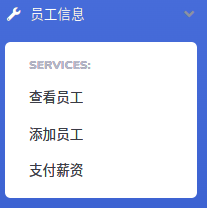
\includegraphics[width=\textwidth]{figures/5employee.png}
%         \subcaption{员工信息二级菜单图}
%         \label{fig:employee}
%     \end{subfigure}
%     \qquad
%     \begin{subfigure}{.25\textwidth}
%         \centering
%         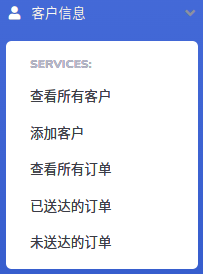
\includegraphics[width=\textwidth]{figures/5customer.png}
%         \subcaption{客户信息二级菜单图}
%         \label{fig:customer}
%     \end{subfigure}
%     \qquad
%     \begin{subfigure}{.25\textwidth}
%         \centering
%         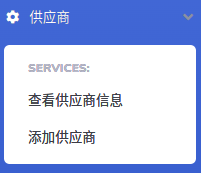
\includegraphics[width=\textwidth]{figures/5supplyer.png}
%         \subcaption{供应商信息二级菜单图}
%         \label{fig:suplier}
%     \end{subfigure}
%     \caption{人员管理类信息管理菜单图}
% \end{figure}

% 点击特定导航栏按钮之后展开的产品与原材料的信息管理操作;如图\ref{fig:product}所示,展示了产品信息的信息管理操作,其中包括查看所有产品以及添加产品操作;如图\ref{fig:raw}所示,展示原材料信息的管理操作。

% \begin{figure}[H]
%     \centering
%     \begin{subfigure}{.25\textwidth}
%         \centering
%         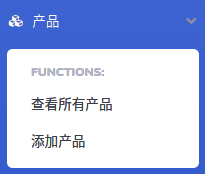
\includegraphics[width=\textwidth]{figures/5product.png}
%         \subcaption{产品信息二级菜单图}
%         \label{fig:product}
%     \end{subfigure}
%     \qquad
%     \begin{subfigure}{.25\textwidth}
%         \centering
%         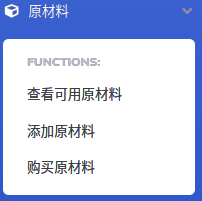
\includegraphics[width=\textwidth]{figures/5raw.png}
%         \subcaption{原材料信息二级菜单图}
%         \label{fig:raw}
%     \end{subfigure}
%     \caption{产品、原材料信息管理菜单图}
% \end{figure}

在信息管理的前端页面中,页面样式导入base基页面为整体样式框架,在div标签元素中,使用table标签将人员信息以表格项的形式进行定义,使用模板语言for标签遍历后端发送的人员数据,将人员信息进行输出展示。在每个表格列末尾,增加与特定人员对应的管理操作,包括修改和删除,使用a标签进行定义,并且将修改后的信息或删除命令发送HTTP请求至后端进行数据实体表的处理。在后端views处理方法中,使用models中定义的数据实体类所对应的表单对象,对信息进行处理,将更新操作保存到数据库中。

管理员可以在后台页面查看当前工厂的人员信息内容,内容以表格的形式呈现,如图\ref{fig:bifmtdf}所示,管理员可以查看当前工厂员工信息表格,并且在此页面可以对员工进行支付薪资、下达工作任务以及删除员工等操作,并且在页面右下方还有计算工资以及添加员工的快捷按钮;与此还有向管理员展示客户信息表格以及供应商信息表格,并且可以通过表格超链接按钮对指定客户进行下单操作以及查看指定客户的订单详情。

\begin{figure}[H]
    \centering
    \begin{subfigure}{.45\textwidth}
        \centering
        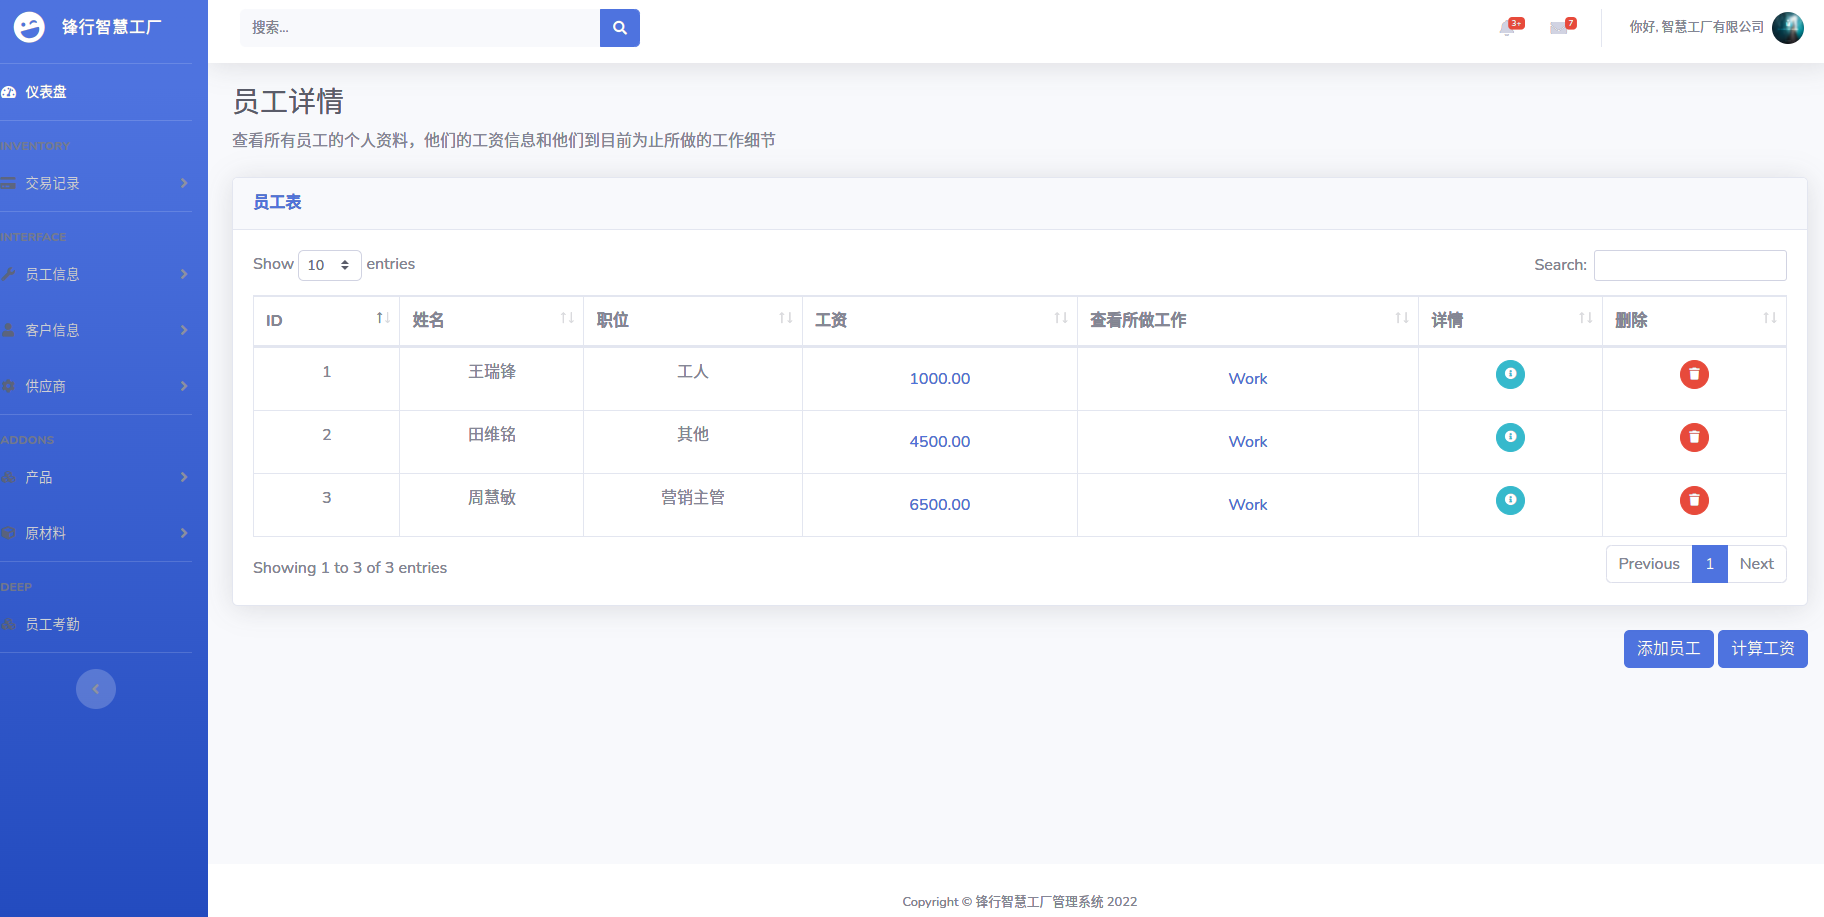
\includegraphics[width=\textwidth]{figures/5employeedetail.png}
        % \subcaption{员工信息详情图}
        % \label{fig:empledtl}
    \end{subfigure}
    \qquad
    \begin{subfigure}{.45\textwidth}
        \centering
        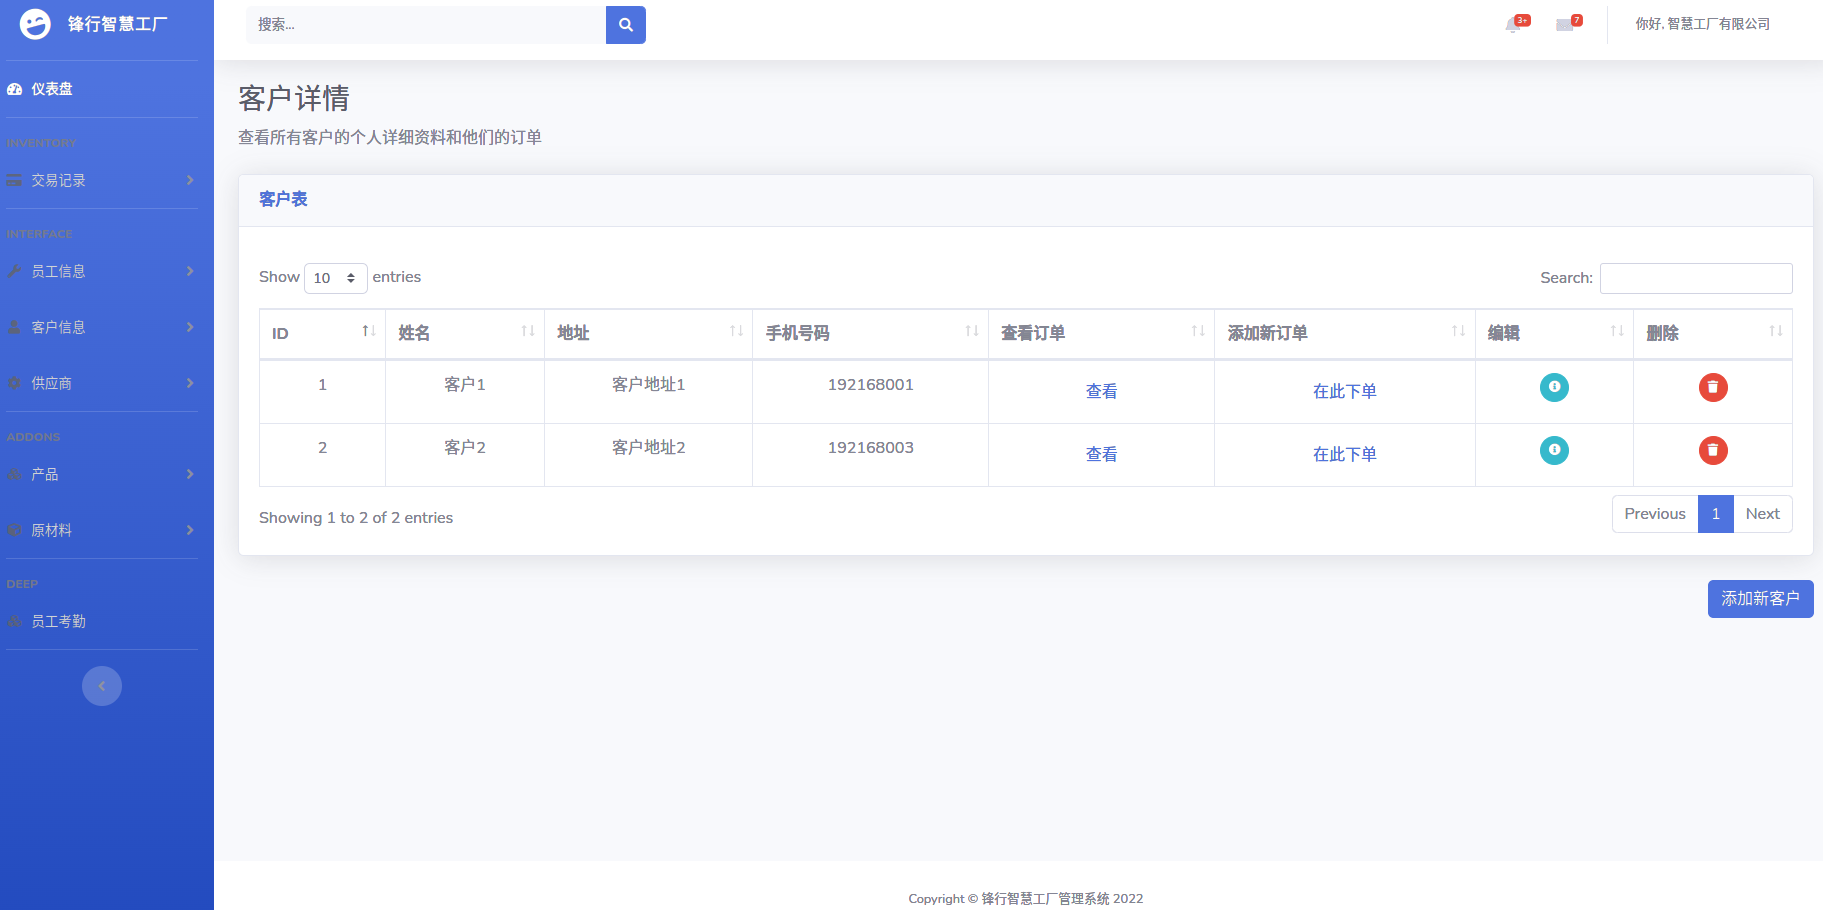
\includegraphics[width=\textwidth]{figures/5customerdetail.png}
        % \subcaption{客户信息详情图}
        % \label{fig:cstmdtl}
    \end{subfigure}
    \\
    \begin{subfigure}{.45\textwidth}
        \centering
        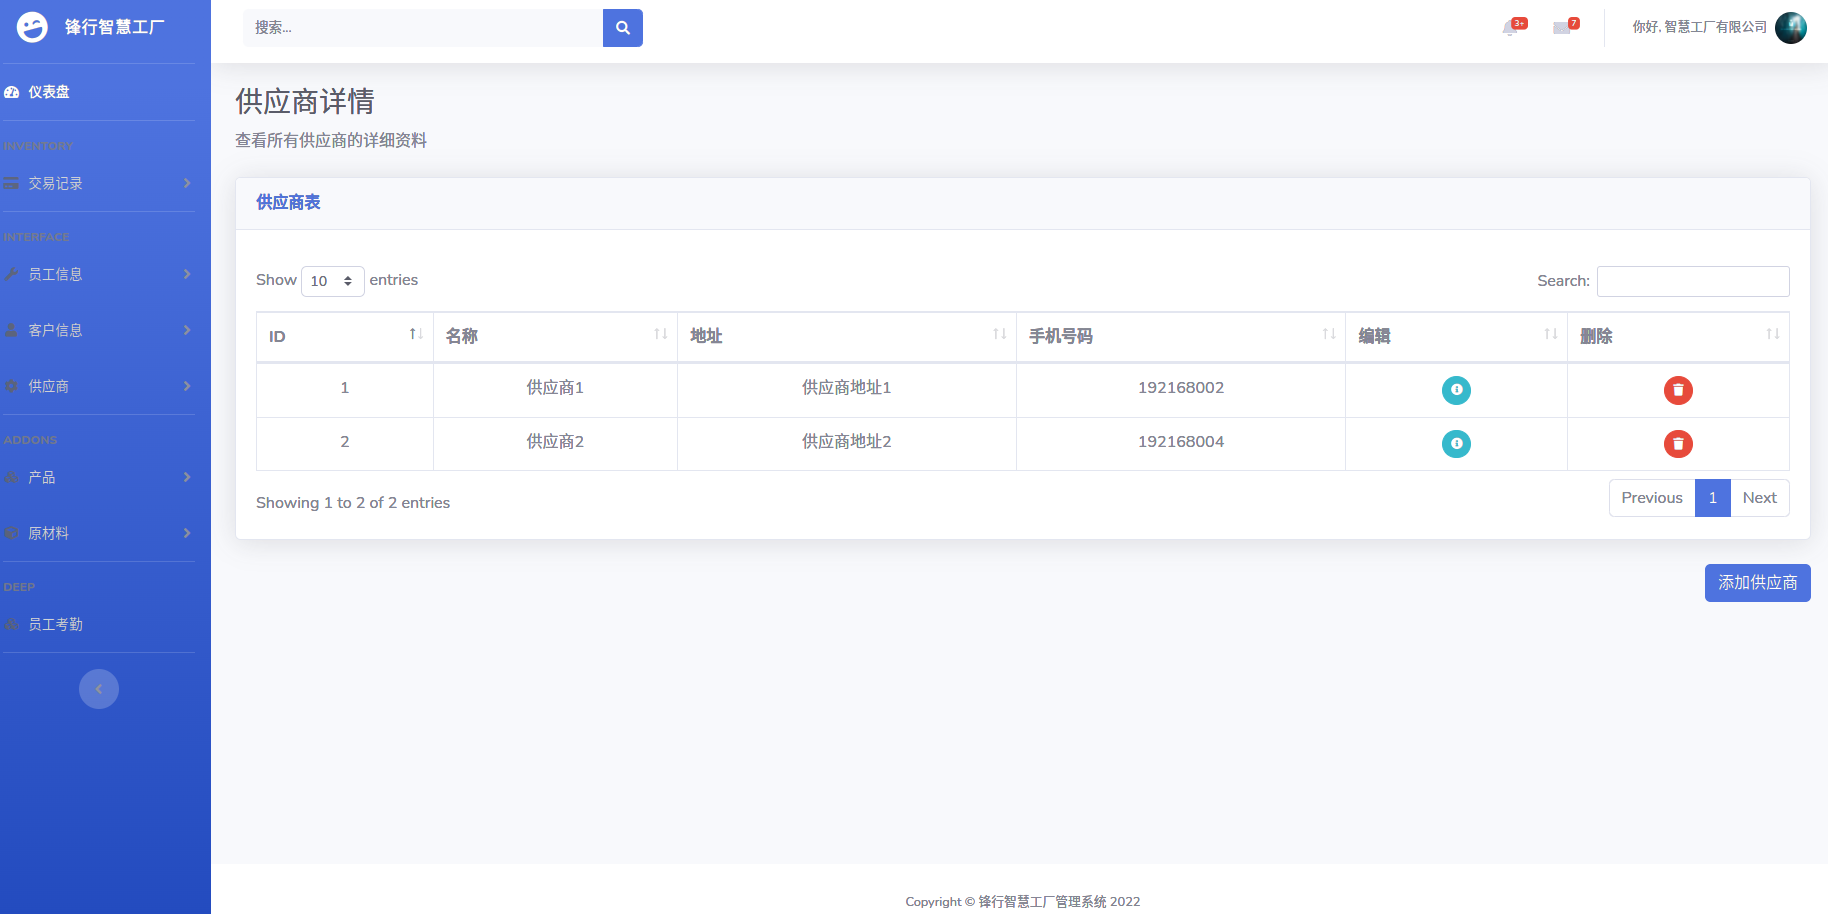
\includegraphics[width=\textwidth]{figures/5supplierdetail.png}
        % \subcaption{供应商信息详情图}
        % \label{fig:spledtl}
    \end{subfigure}
    \qquad
    \begin{subfigure}{.45\textwidth}
        \centering
        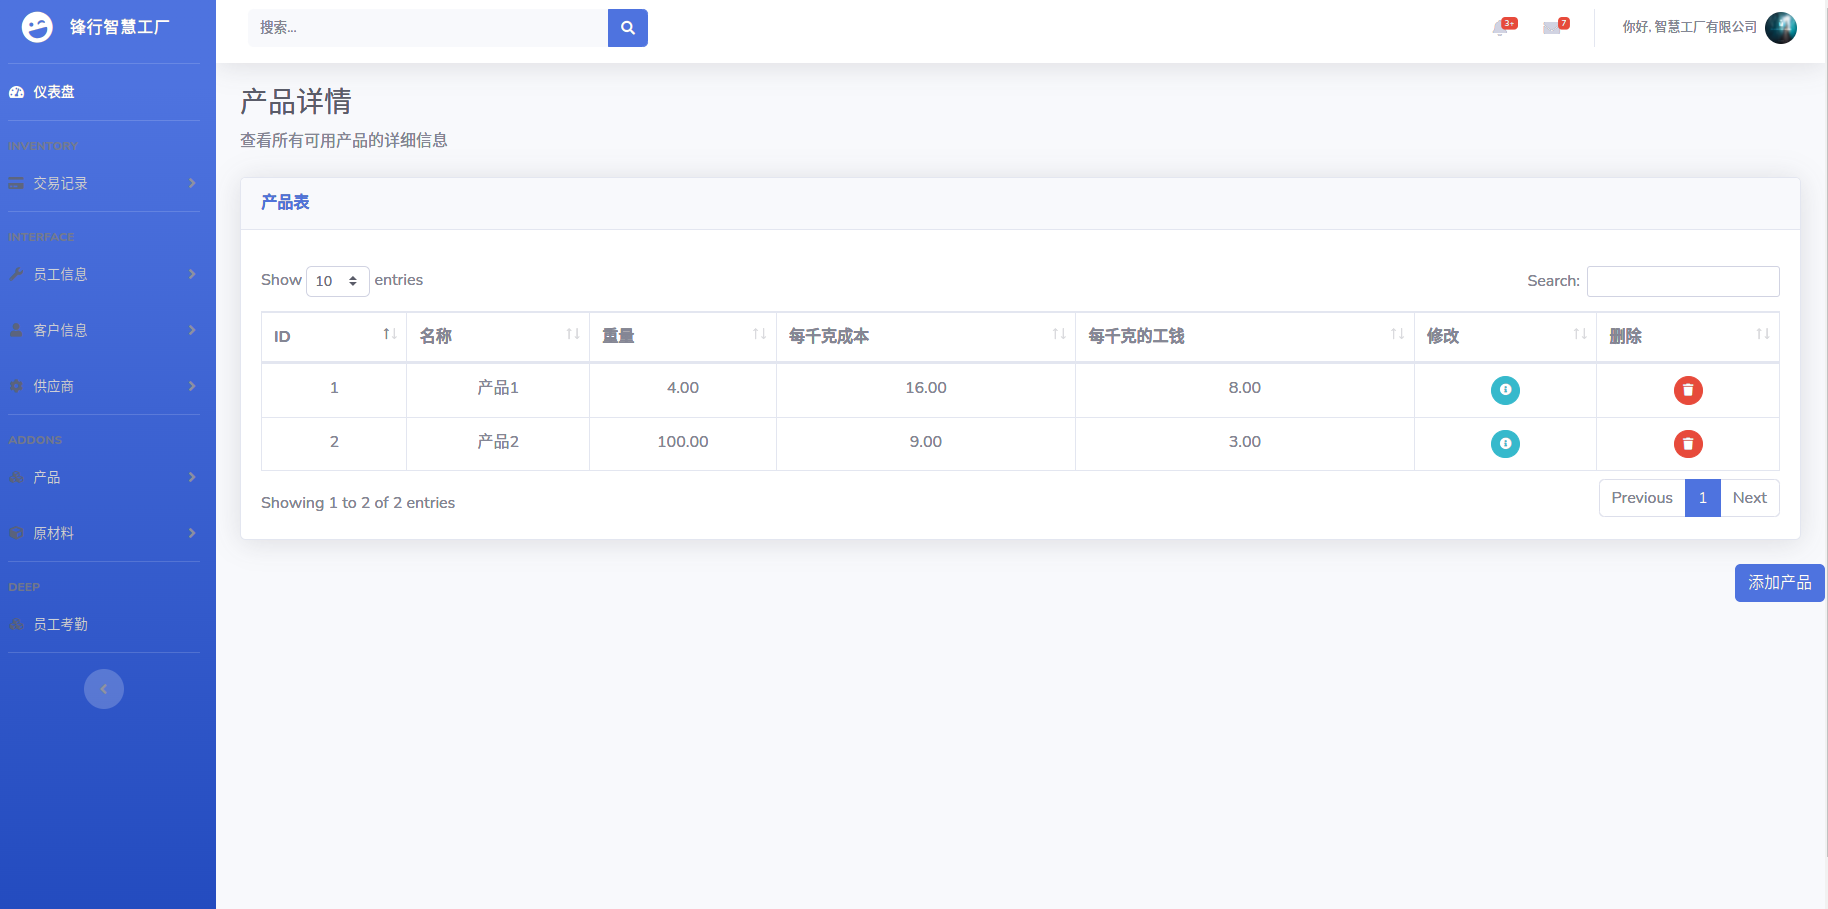
\includegraphics[width=\textwidth]{figures/5productdetail.png}
        % \subcaption{产品信息详情图}
        % \label{fig:prdctdtl}
    \end{subfigure}
    \caption{后台信息管理详情图图}
    \label{fig:bifmtdf}
\end{figure}

\subsubsection{员工考勤功能实现}

工厂管理员进入到员工考勤页面,向管理员展示一个员工签到记录表,查看员工的签到记录以及签到时间。首先在员工考勤页面加载base基页面,使用div标签元素定义员工签到记录内容展示,使用模板语言for标签遍历后端发送来的员工签到记录,将记录以表格的形式进行输出展示。在后端views模块中处理HTTP请求方法内,使用数据访问对象获取到全部签到表记录封装至签到字典变量中,通过HTTP响应发送至前端。如图\ref{fig:empleatd}所示,展示了员工签到记录表。并且在上方有一个人脸识别签到的按钮,以供员工以人脸识别的方式进行签到。

\begin{figure}[H]
    \centering
    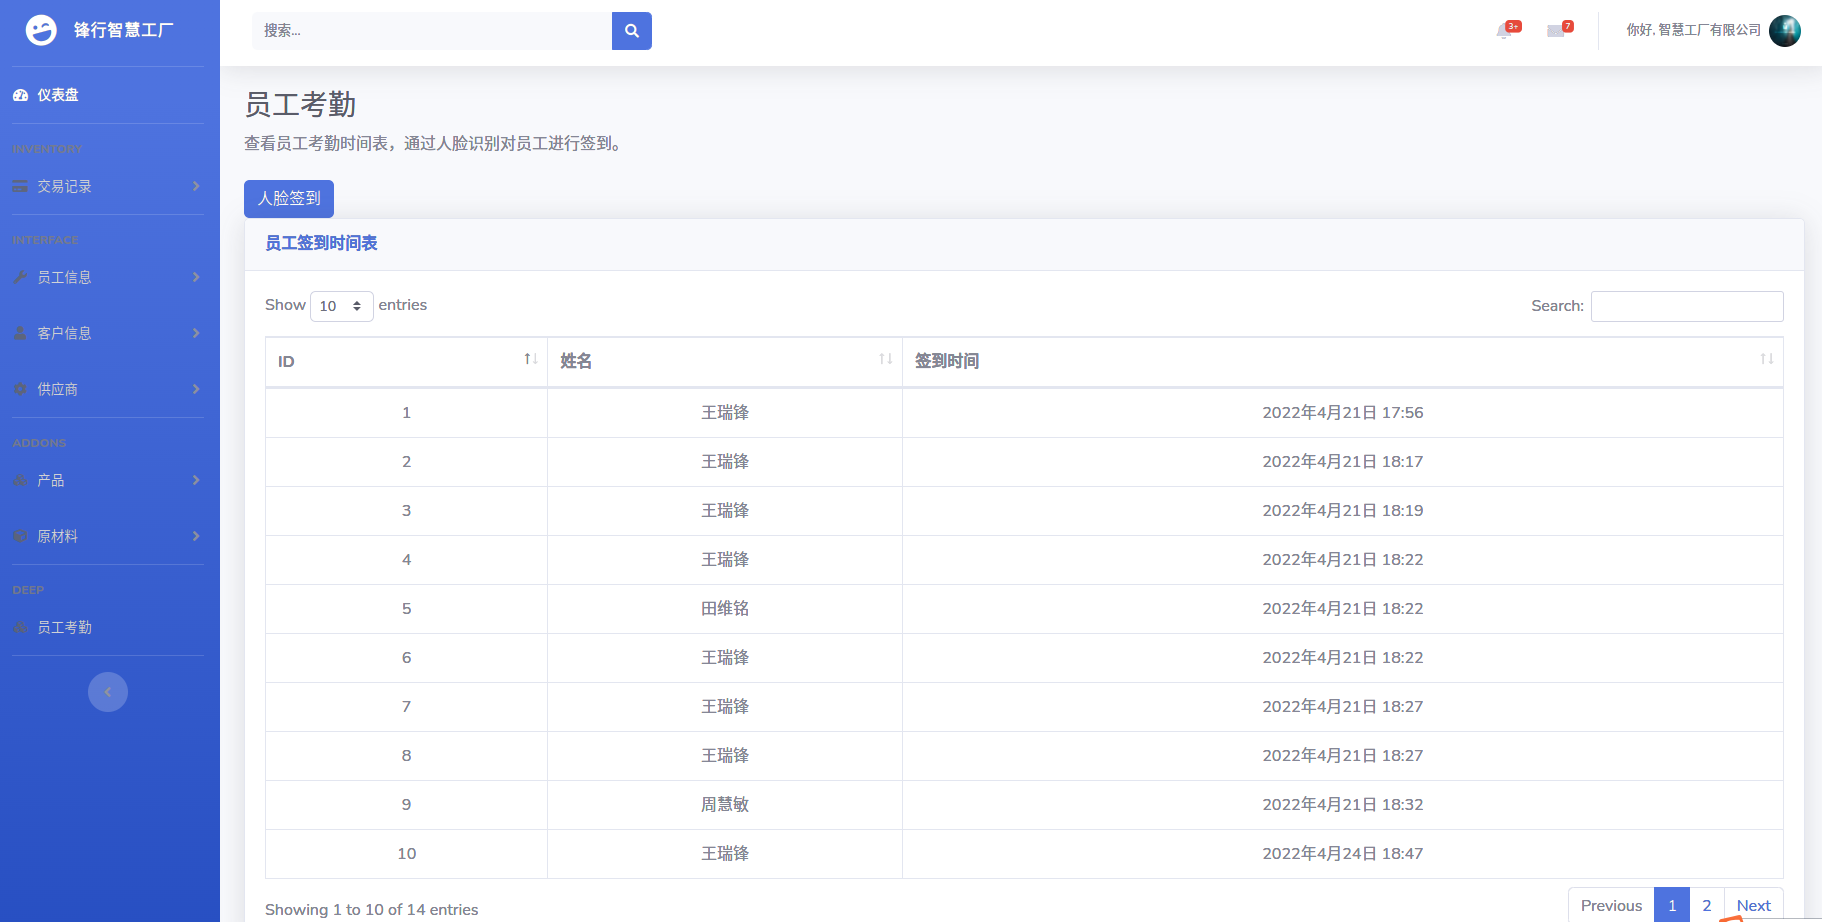
\includegraphics[width=.75\textwidth]{figures/5empleatd.png}
    \caption{员工考勤签到记录详情图}
    \label{fig:empleatd}
\end{figure}

\subsection{人脸识别签到功能实现}

随着社会的发展,信息化时代已经来临,人脸识别技术的不断成熟,基于人脸识别的签到系统也不断出现,基于本地的人脸识别签到考勤系统的需求也很迫切,基于此,本系统设计了一个人脸识别签到系统。工厂管理员进入后台页面,可以使用人脸识别模块对当前员工进行,通过比较阈值之后,将识别到的员工信息与签到时间插入到员工签到记录表中,具体流程如图\ref{fig:fcprcs}所示。

\begin{figure}[H]
    \centering
    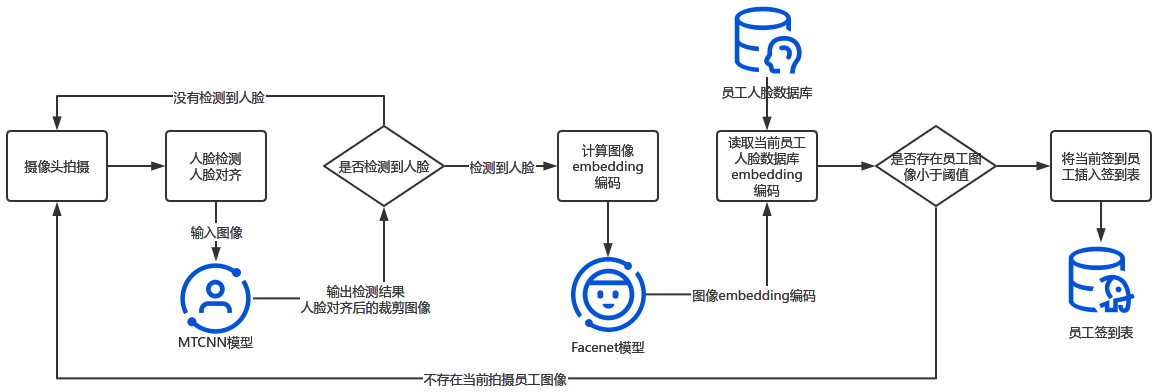
\includegraphics[width=\textwidth]{figures/5fcprcs.png}
    \caption{人脸识别签到流程图}
    \label{fig:fcprcs}
\end{figure}

当系统管理员调用人脸识别签到功能时,该模块首先从摄像头拍摄图像,将图像输入进MTCNN模型来对图像中的人脸进行检测,若没有检测到人脸,便从系统中弹出拍摄框并且回到摄像头拍摄进行重新拍摄;若检测到人脸存在,就将人脸区域的图像进行裁剪,裁剪的尺寸为160$\times$160的像素;将裁剪后的人脸图像输入进MaskedFacenet网络模型中,计算当前人脸图像的embedding编码;之后将系统中保存的员工人脸图像的embedding编码与刚刚计算的人脸图像embedding编码进行比较,计算二者们的$L_2$范数,也即两者之间在欧式空间中的距离,之后挑选出距离最小的图像对,换句话说也就是相似度最高的员工图像,然后使用阈值比较,本文使用的阈值为1,若小于这个阈值,便判定为当前拍摄的员工为人脸数据库中的员工,之后便将签到时间与员工信息插入到员工签到记录表中,便实现了人脸识别签到功能。

\subsubsection{模型训练}

本系统选用预训练的MTCNN网络模型作为人脸识别系统中的人脸检测与人脸对齐模块,选用基于CASIA-Webface人脸数据集预训练的Facenet网络模型。为了提升佩戴口罩的人脸识别准确率,本文使用MaskTheFace工具对CASIA-Webface人脸数据集进行模拟佩戴口罩来构造训练数据集CASIA-Webmaskedface用于微调模型,如图\ref{fig:cmrsds}所示,为了作为对比,左图为原CASIA-Webface人脸数据集,右图为使用MaskTheFace工具模拟佩戴口罩后的人脸数据集CASIA-Webmaskedface。构造后的CASIA-Webmaskedface模拟佩戴口罩人脸数据集有10,575位人物共494,414张人脸图像。

\begin{figure}[H]
    \centering
    \begin{subfigure}{.45\textwidth}
        \centering
        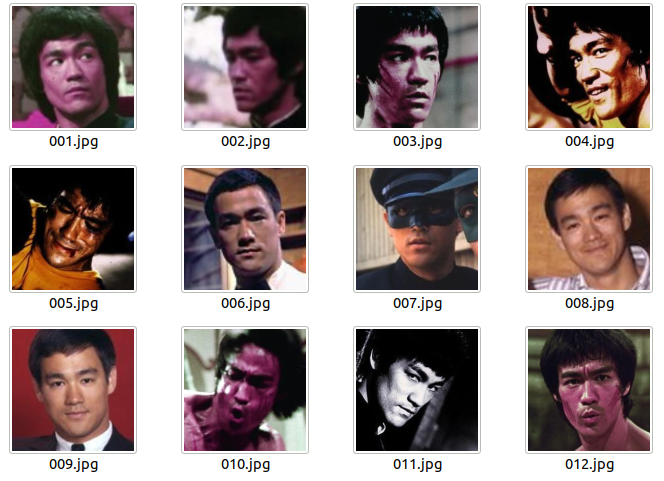
\includegraphics[width=\textwidth]{figures/4webface.png}
        % \subcaption{原CASIA-Webface人脸数据集样本图}
        % \label{fig:owebface}
    \end{subfigure}
    \qquad
    \begin{subfigure}{.45\textwidth}
        \centering
        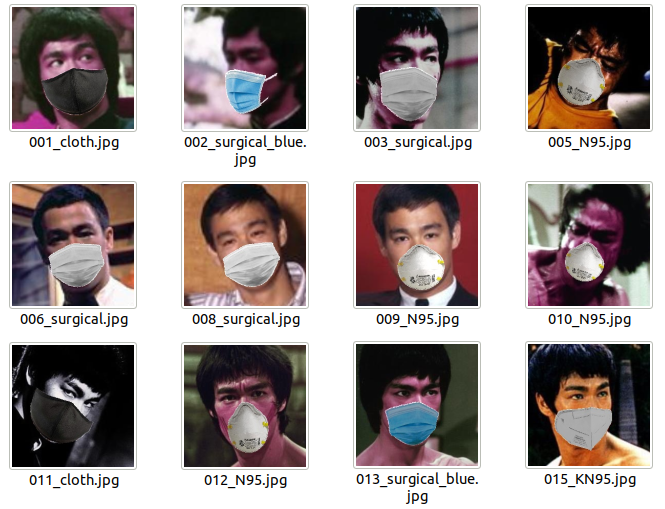
\includegraphics[width=\textwidth]{figures/5webmaskedface.png}
        % \subcaption{模拟佩戴口罩数据集样本图}
        % \label{fig:webmakedface}
    \end{subfigure}
    \caption{模拟佩戴口罩人脸数据集对比图}
    \label{fig:cmrsds}
\end{figure}

Facenet网络模型的骨干架构使用的是Inception Resnet V1模型,该模型的网络架构如图\ref{fig:resnetarc}所示。其中输入为$160\times 160$的剪裁后的人脸图像,输出为512维的图像embedding编码。

\begin{figure}[H]
    \centering
    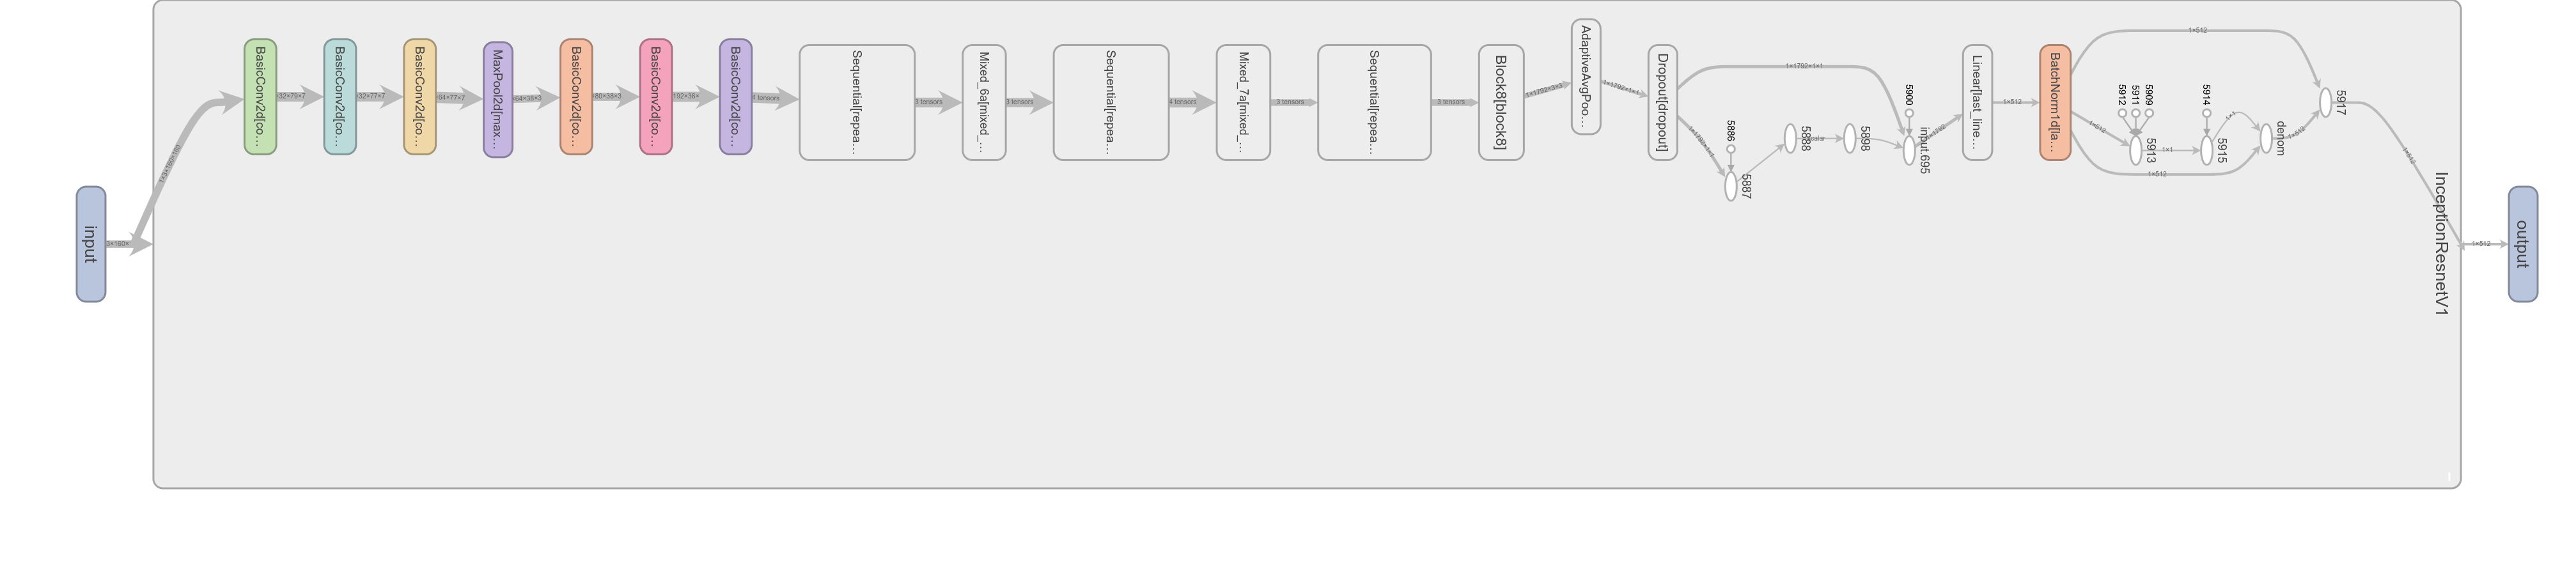
\includegraphics[width=\textwidth]{figures/5modelarc.png}
    \caption{Inception Resnet V1模型架构图}
    \label{fig:resnetarc}
\end{figure}

\subsubsection{模型参数}

本系统使用的Facenet网络模型的参数数量如表\ref{tab:modelparams}所示,其中该网络模型前三层为卷积层、一个最大化池化层、之后继续为3个卷积层。随后跟着2对repeat与mixed模块,其中repeat模块中包含了若干数量的Block块,每个Block块都含有并行的卷积层与残差模块结合,使用ReLU激活函数;mixed模块中包含了将若干数量的卷积层与最大化池化层并行传输。之后为调整的平均池化层与Dropout层用来防止过拟合,其中Dropout的概率为0.6。最后跟着一个全连接层将输出映射为512维向量,然后跟着一个Batchnorm将输出进行规范化,最后输出为512维的embedding编码。该网络模型共23,482,624个用于训练的参数。

\begin{table}[H]
    \zihao{5}
    \centering
    \caption{Facenet网络模型参数量表}
    \label{tab:modelparams}
    \begin{tabularx}{.95\textwidth}{X<{\centering}X<{\centering}X<{\centering}}
    % \begin{tabular}{rrr}
        \toprule
        Layer (type)          & Output Shape     & Param \# \\
        \midrule
        Conv2d-1              & [-1, 32, 79, 79] & 864      \\
        BatchNorm2d-2         & [-1, 32, 79, 79] & 64       \\
        ReLU-3                & [-1, 32, 79, 79] & 0        \\
        BasicConv2d-4         & [-1, 32, 79, 79] & 0        \\
        Conv2d-5              & [-1, 32, 77, 77] & 9,216    \\
        BatchNorm2d-6         & [-1, 32, 77, 77] & 64       \\
        ReLU-7                & [-1, 32, 77, 77] & 0        \\
        $\vdots$              & $\vdots$         & $\vdots$ \\
        BasicConv2d-509       & [-1, 192, 3, 3]  & 0        \\
        Conv2d-510            & [-1, 1792, 3, 3] & 689,920  \\
        Block8-511            & [-1, 1792, 3, 3] & 0        \\
        AdaptiveAvgPool2d-512 & [-1, 1792, 1, 1] & 0        \\
        Dropout-513           & [-1, 1792, 1, 1] & 0        \\
        Linear-514            & [-1, 512]        & 917,504  \\
        BatchNorm1d-515       & [-1, 512]        & 1,024    \\
        % \midrule
        % Total params:         & 23,482,624       &          \\
        % Trainable params:     & 23,482,624       &          \\
        % Non-trainable params: & 0                &          \\
        \bottomrule
    \end{tabularx}
\end{table}

关于超参数方面,在本系统使用的Facenet网络模型中,batch size(数据批量大小)为64,训练集与验证集之比为8:2;优化算法使用Adam算法,其中学习率$\gamma$为0.001、$\beta_{1}$为0.9、$\beta_{2}$为0.999、$\epsilon$为1e-08、$\lambda$(weight decay)为0;学习率调度算法为MultiStepLR,其中milestone区间为$(5,10)$、$\gamma$为0.1;最后,在整个训练集之上训练的epoch次数为8。关于数据增强(data augmentation)方面,由于本文所使用的训练数据集足够大,所以并没有做数据增强方面的工作,仅把图像像素值标准化。

在训练过程,模型的准确率与损失值如图\ref{fig:mdmtx}所示,左图为模型准确率变化,右图为损失值变化。最终模型在训练集上的准确率94.29\%为,损失值为0.3336;在验证集上的准确率为80.04\%,损失值为1.3949。

\begin{figure}[H]
    \centering
    \begin{subfigure}{.45\textwidth}
        \centering
        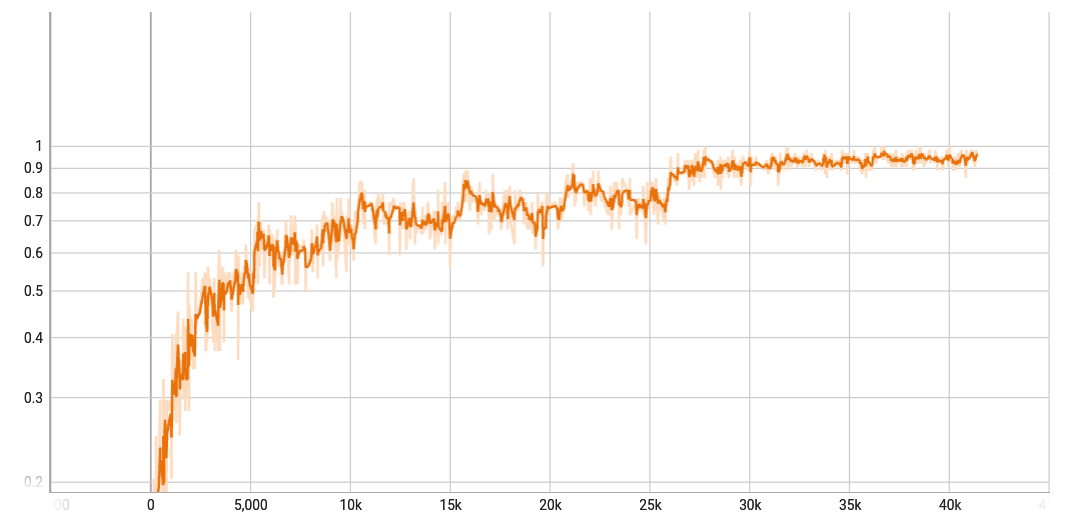
\includegraphics[width=\textwidth]{figures/5acc.png}
        % \subcaption{模型训练阶段准确率图}
        % \label{fig:acc}
    \end{subfigure}
    \qquad
    \begin{subfigure}{.45\textwidth}
        \centering
        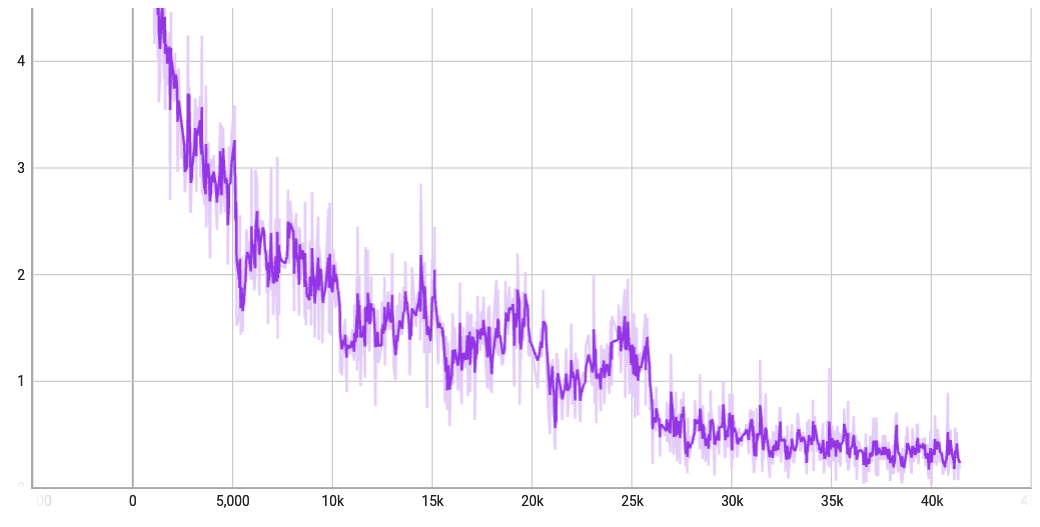
\includegraphics[width=\textwidth]{figures/5loss.png}
        % \subcaption{模型训练阶段损失值图}
        % \label{fig:loss}
    \end{subfigure}
    \caption{模型训练阶段性能指标图}
    \label{fig:mdmtx}
\end{figure}

\subsubsection{模型评估}

当预训练的Facenet模型在CASIA-Webmaskedface模拟佩戴口罩人脸数据集上训练了8个epoch之后,使用LFW与MFR2测试数据集进行模型性能的比较。如表\ref{tab:mdcprs}所示,原Facenet网络模型在LFW与MFR2测试数据的准确率为表格中的第一行,使用了CASIA-Webmaskedface模拟佩戴口罩人脸数据集微调(finetune)之后,MaskedFacenet在LFW与MFR2测试数据集上的模型性能为表格中的第二行。可以看到,使用了CASIA-Webmaskedface模拟佩戴口罩人脸数据集对模型进行微调之后,该模型在LFW人脸测试数据集的准确率稍微有点下降,但是对于真实世界环境中的佩戴口罩人脸数据集MFR2却有了很大的提升,在MFR2测试数据集上的准确率有95.27\%的准确率,相比较与Facenet网络模型提升了6.14\%的准确率。所以本系统所使用的网络模型在佩戴口罩的情况下对人脸识别的准确率有着比较大的提升空间。

\begin{table}[H]
    \zihao{5}
    \centering
    \caption{网络模型性能比较表}
    \label{tab:mdcprs}
    \begin{tabularx}{.95\textwidth}{X<{\centering}X<{\centering}X<{\centering}}
    % \begin{tabular}{rrr}
        \toprule
        模型 & LFW准确率 & MFR2准确率 \\
        \midrule
        Facenet & 98.53\% & 89.13\% \\
        MaskedFacenet & 95.43\% & 95.27\% \\
        \bottomrule
    \end{tabularx}
\end{table}
